\begin{section}{Power Spectra and Information Content}
  \label{sec:fisherinfo}
    The power spectrum is the Fourier transform of the correlation function and measures the amoutn of clustering in the matter distribution in terms of the wavenumber $k$ in unit of $h \mathrm{Mpc}^{-1}$,
\begin{align}
    \langle \delta \left( \bm{k} \right) \delta \left( \bm{k'}\right) \rangle =\left( 2\pi \right) ^3 P \left( \bm{k} \right) \hat{\delta} \left( \bm{k}-\bm{k'} \right),
\end{align}
where $\delta \left( \bm{k} \right)$ is the density fluctuation in wave space, while $\hat{\delta}$ is the delta funciton. Of equal interest is $\Delta ^2_k$, the power spectrum in its dimensionless form, defined as
\begin{align}
    \Delta ^2_k \equiv \frac{k^3 P \left( k \right)}{2\pi ^2}
\end{align}
    The power spectra of the mass distributions are calculated using the "Nearest Grid Point" (NGP) mass assignment scheme, which calculates the position of each particle based on which grid point it is nearest. In Fig.... we plot the mean power spectrum (and error bars) of 139 density fields and reconstruced deformation potentials.
    To calculate the cumulative Fisher information of the density fields, the covariance matrix of the power spectra should be first given. Mathematically, the the covariance matrix is defined as
\begin{align}
    \mathrm{Cov}\left(k,k'\right)\equiv \frac{1}{N-1}\sum_{i=1}^{N}\left[ P_i \left( k \right) - \langle P \left( k \right) \rangle \right]\left[ P_j \left( k' \right) - \langle P \left( k' \right)\rangle \right],
\end{align}
where angle brackets mean the expected values. 
    The cross-correlation coefficient matrix, or for short, the correlation matrix, is a normalized version of the covariance matrix,
\begin{align}
    \mathrm{Corr}\left(k,k'\right)=\frac{\mathrm{Cov}\left(k,k'\right)}{\sqrt{\mathrm{Cov}\left(k,k\right)\mathrm{Cov}\left(k',k'\right)}}.
\end{align}
The corelation matrices for density fields from simulations and deformation potentials from reconstructions are shown in Fig. \ref{fig:corrall}. For the original density fields, the linear regime, where $k<0.1$, is diagonal, while in the non-linear regime, the power spectra of different $k$ modes are strongly correlated by at least $60\%$ . For the reconstructed deformation potential correlation matrix, however, the linear regime expand up to $k~0.2$. The correlation matrix is closer to that for the power spectra of linear density fields.
\begin{figure}
 \centering
% \begin{subfigure*}[b]{0.5\textwidth}
% \centering
  \includegraphics[width=0.5\textwidth]{corr2-crop.pdf}
%\label{fig:corrnb}
% \end{subfigure*}
% \begin{subfigure*}[b]{0.5\textwidth}
% \centering
%  \includegraphics[width=0.45\textwidth]{corrrecnew-crop.pdf}
%\label{fig:corrrec}
% \end{subfigure*}
%\begin{subfigure}
%\begin{figure}
%  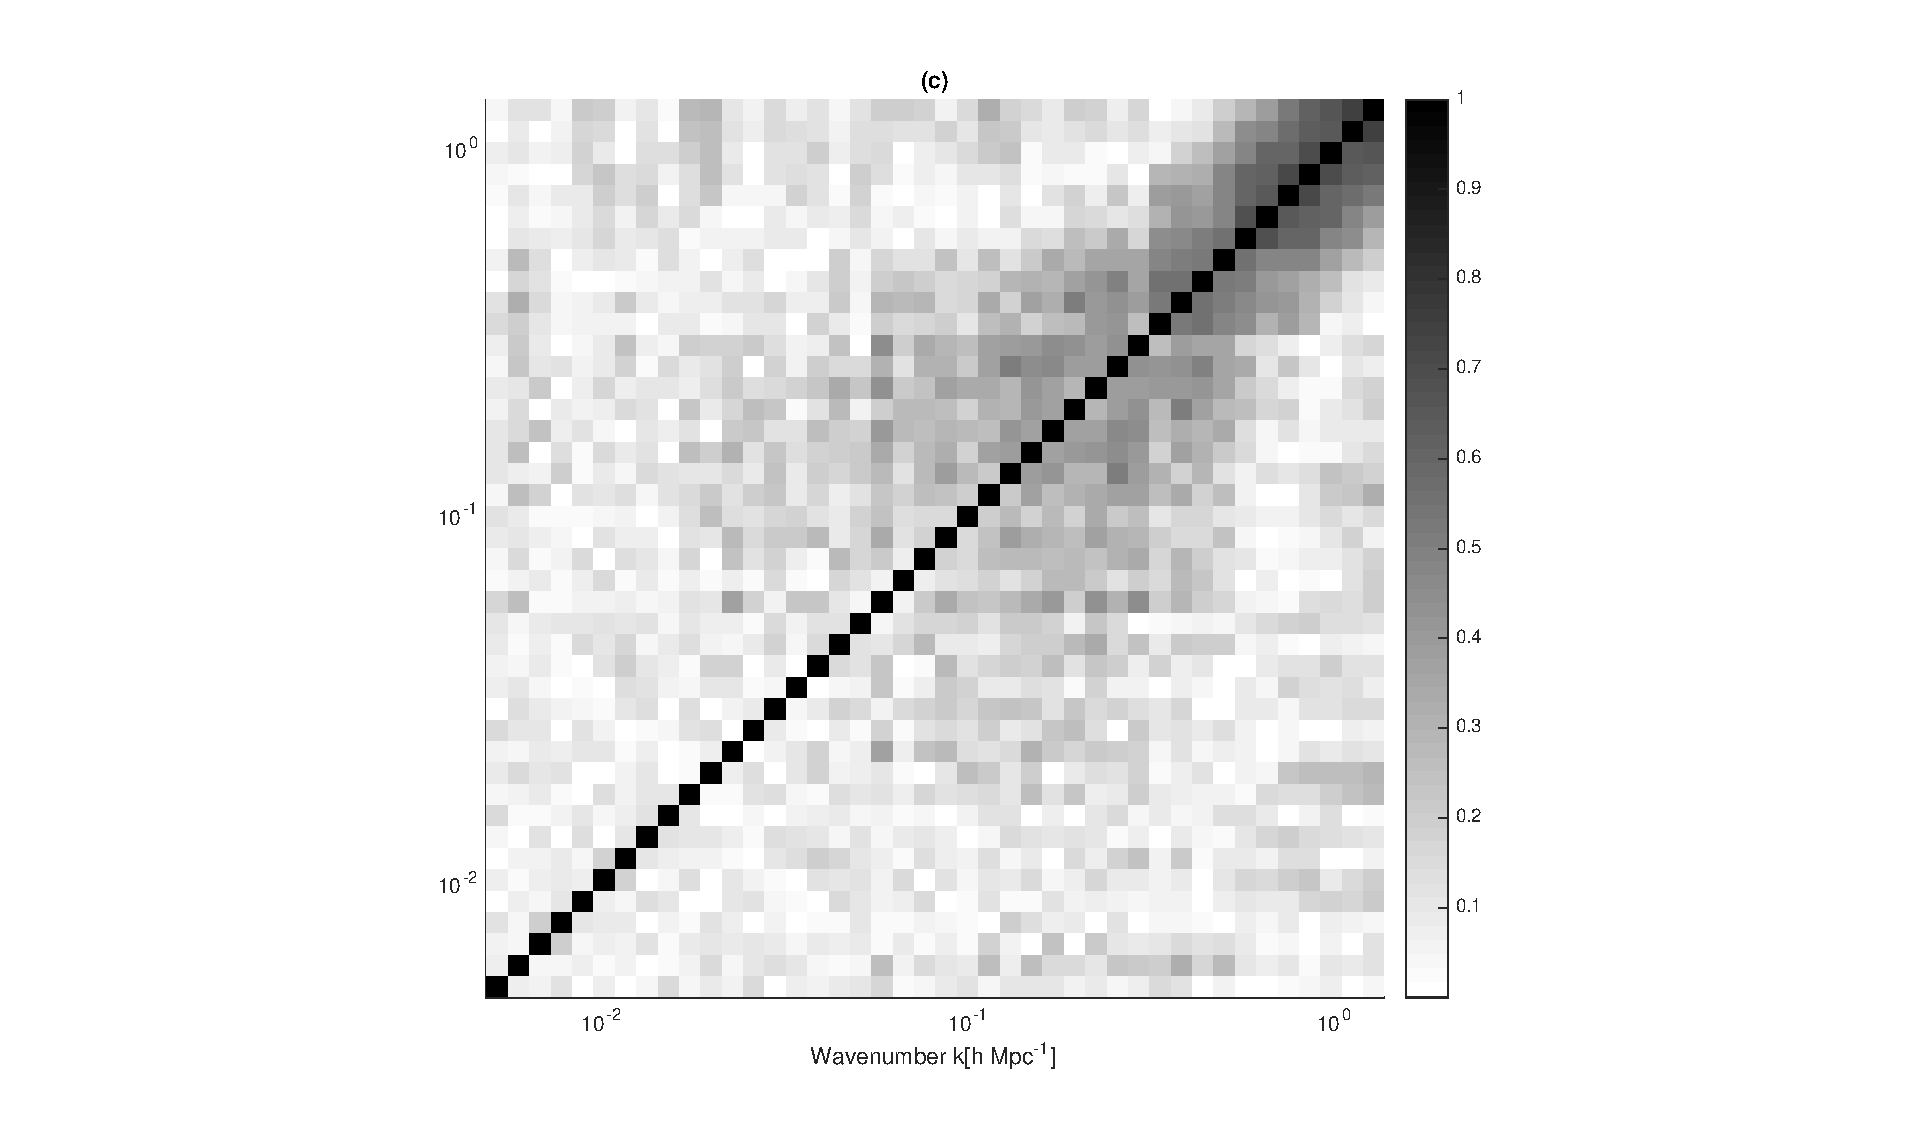
\includegraphics[width=0.5\textwidth]{corrlin.eps}
% \end{subfigure}
%\begin{figure}
%    \centering
%    \includegraphics[width=\textwidth,height=0.5\textwidth]{corrall.eps}
%
  \caption{Cross-correlation coefficient matrix as found from 136 power spectra of the non-linear density field from simulation (the upper triangle) and the deformation potential field from reconstruction(the lower triangle).}   

    \label{fig:corrall}
\end{figure}
    The cumulative, or Fisher, information function of $k_n$ is then defined as the sum of the elements of inverse of subsection of the normalized covariance matrix up to $k_n$ scale
\begin{align}
    I \left( < k_n\right) = \sum_{i,j=1}^n \left[ C^{-1}_{norm} \left( k_i,k_j \right)\right] \left( i,j \leq n \right),
\end{align}
where $C_{norm}$ is the normalized covariance matrix, defined as
\begin{align}
    C_{norm} \left( k,k' \right)=\frac{\mathrm{Cov}(k,k')}{\langle P(k)\rangle\langle P(k)\rangle}.
\end{align}
  
%  The signal-to-noise ratio, sometimes also called Fisher information, can be given by the inverse matrix of covariance. Since the signal-to-noise ratio was given in some work, we also present it for a better comparison. 
%\begin{align}
%\left( \frac{S}{N}\right)^2 (k_{n}) =\sum_{i,j=1}^n P_i \mathrm{Cov}^{-1}(i,j) P_j
%\end{align}
As seen above, cumulative information is a measurement of the number of independent Fourier modes presented in a field up to a given $k_n$, which represents how linear a field is. We plot the cumulative information of the power specta of density fields from simulations and deformation potentials from reconstructions in Fig.\ref{fig:fisherinfo}. In the translinear regime, where $k\sim0.1$, the cumulative information of the non-linear density field has a flat plateau. It indicates that there's nearly no independent information in the translinear regime of the power spectrum. At $k\sim0.8$, the information increase slightly aggain. But the information curve of the reconstructed deformation potential keeps incresing and reaches it's plateau at $k\sim0.6-0.7$ up to a factor of 20. It indicates that APM method can strongly recover the lost information within this scale. 
\begin{figure}[htbp]
 \begin{center}
  \includegraphics[width=0.5\textwidth]{fishernew-crop.pdf}
   \caption{Cumulative information in the power spectra as a function of wavenumber. The blue cycles correspond to the non-linear density field by simulation; the black squares correspond to the the reconstructed deformation potential; the red dash line corresponds to linear density field at $z=0$; the green crosses correspond to linear density field at $z=100$.}
  \label{fig:fisherinfo}
 \end{center}
\end{figure}


\end{section}
